% Construction : f(x) = (2x − 1)e^{−2x+3} sur [0,5 ; 3,3]. La fonction s'annule
% en 0,5, atteint son maximum e en x = 1, puis décroît. L'aire hachurée, entre
% ces deux bornes, vaut 0,5e² − 3,3e^{−3,6}, soit 3,6 au dixième.
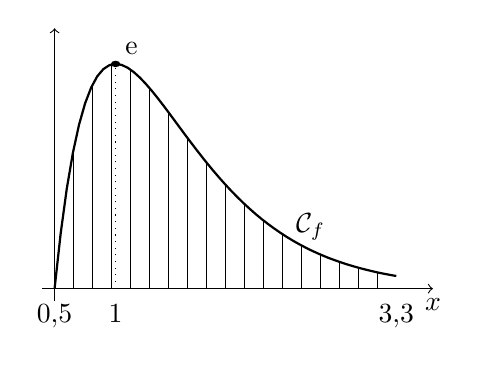
\begin{tikzpicture}[xscale=1.55, yscale=1.05]
  \draw[->] (0.4, 0) -- (3.6, 0) node[below] {$x$};
  \draw[->] (0.5, -0.15) -- (0.5, 3.15);
  \draw[thin] (0.656, 0) -- (0.656, 1.684);
  \draw[thin] (0.811, 0) -- (0.811, 2.468);
  \draw[thin] (0.967, 0) -- (0.967, 2.712);
  \draw[thin] (1.122, 0) -- (1.122, 2.649);
  \draw[thin] (1.278, 0) -- (1.278, 2.426);
  \draw[thin] (1.433, 0) -- (1.433, 2.133);
  \draw[thin] (1.589, 0) -- (1.589, 1.823);
  \draw[thin] (1.744, 0) -- (1.744, 1.526);
  \draw[thin] (1.900, 0) -- (1.900, 1.258);
  \draw[thin] (2.056, 0) -- (2.056, 1.024);
  \draw[thin] (2.211, 0) -- (2.211, 0.825);
  \draw[thin] (2.367, 0) -- (2.367, 0.660);
  \draw[thin] (2.522, 0) -- (2.522, 0.524);
  \draw[thin] (2.678, 0) -- (2.678, 0.413);
  \draw[thin] (2.833, 0) -- (2.833, 0.324);
  \draw[thin] (2.989, 0) -- (2.989, 0.253);
  \draw[thin] (3.144, 0) -- (3.144, 0.197);
  \draw[thick] plot coordinates {(0.500, 0.000) (0.550, 0.669) (0.600, 1.210) (0.650, 1.642) (0.700, 1.981) (0.750, 2.241) (0.800, 2.433) (0.850, 2.569) (0.900, 2.656) (0.950, 2.704) (1.000, 2.718) (1.050, 2.706) (1.100, 2.671) (1.150, 2.618) (1.200, 2.551) (1.250, 2.473) (1.300, 2.387) (1.350, 2.295) (1.400, 2.199) (1.450, 2.100) (1.500, 2.000) (1.550, 1.900) (1.600, 1.801) (1.650, 1.704) (1.700, 1.609) (1.750, 1.516) (1.800, 1.427) (1.850, 1.341) (1.900, 1.258) (1.950, 1.179) (2.000, 1.104) (2.050, 1.032) (2.100, 0.964) (2.150, 0.899) (2.200, 0.838) (2.250, 0.781) (2.300, 0.727) (2.350, 0.676) (2.400, 0.628) (2.450, 0.583) (2.500, 0.541) (2.550, 0.502) (2.600, 0.465) (2.650, 0.431) (2.700, 0.399) (2.750, 0.369) (2.800, 0.342) (2.850, 0.316) (2.900, 0.292) (2.950, 0.270) (3.000, 0.249) (3.050, 0.230) (3.100, 0.212) (3.150, 0.195) (3.200, 0.180) (3.250, 0.166) (3.300, 0.153)};
  \draw[dotted] (1, 0) -- (1, 2.718);
  \fill (1, 2.718) circle (1.1pt);
  \node[below] at (0.5, -0.08) {$0{,}5$};
  \node[below] at (1, -0.08) {$1$};
  \node[below] at (3.3, -0.08) {$3{,}3$};
  \node[above right] at (1, 2.718) {$\mathrm{e}$};
  \node[right] at (2.4, 0.75) {$\mathcal{C}_f$};
\end{tikzpicture}
